\documentclass[aspectratio=169,11pt]{beamer}
\usepackage[utf8]{inputenc}
\usepackage[T1]{fontenc}
\usepackage[english]{babel}
\usepackage{amsmath,amssymb,booktabs,array,listings,xcolor,graphicx}

\usetheme{default}
\definecolor{navy}{HTML}{17324D}
\definecolor{rust}{HTML}{B64B35}
\definecolor{sand}{HTML}{F4E9D8}
\definecolor{ink}{HTML}{1E252B}
\definecolor{muted}{HTML}{60717E}
\setbeamercolor{normal text}{fg=ink,bg=white}
\setbeamercolor{frametitle}{fg=navy,bg=white}
\setbeamercolor{structure}{fg=rust}
\setbeamercolor{alerted text}{fg=rust}
\setbeamerfont{frametitle}{size=\Large,series=\bfseries}
\setbeamerfont{title}{size=\LARGE,series=\bfseries}
\setbeamertemplate{navigation symbols}{}
\setbeamertemplate{footline}{%
  \hfill\usebeamerfont{page number in head/foot}\insertframenumber\hspace{0.45cm}\vspace{0.18cm}}
\setbeamersize{text margin left=0.7cm,text margin right=0.7cm}

\lstdefinelanguage{Lean}{
  keywords={def,theorem,lemma,structure,where,by,have,exact,simpa,using,let,if,then,else,Prop,Real},
  sensitive=true,
  morecomment=[l]{--},
  morestring=[b]"
}
\lstset{
  language=Lean,
  basicstyle=\ttfamily\scriptsize,
  keywordstyle=\color{navy}\bfseries,
  commentstyle=\color{muted},
  columns=fullflexible,
  keepspaces=true,
  frame=single,
  rulecolor=\color{sand},
  breaklines=true,
  showstringspaces=false
}

\newcommand{\source}[1]{\vfill{\tiny\color{muted}Source: #1}}
\newcommand{\paper}{\textcolor{navy}{\textbf{PAPER}}}
\newcommand{\derivation}{\textcolor{rust}{\textbf{DERIVATION}}}
\newcommand{\interpretation}{\textcolor{muted}{\textbf{INTERPRETATION}}}

\title{Acemoglu \& Restrepo (2018)}
\subtitle{The race between automation and new tasks}
\author{Alvaro Marcelo Ch\'avez Unyen}
\date{Repository 6 · September 24, 2026}

\begin{document}

\begin{frame}[plain]
  \vspace{0.5cm}
  {\usebeamerfont{title}\color{navy}\inserttitle\par}
  \vspace{0.2cm}
  {\large\insertsubtitle\par}
  \vspace{0.55cm}
  {\normalsize\insertauthor\par}
  {\small\insertdate\par}
  \vfill
  {\small\color{rust}\texttt{github.com/amchavezu/ai-06-restrepo}}
  \vspace{0.35cm}
  {\tiny\color{muted}NBER Working Paper 22252, revised June 2017. Proposition numbering follows this version.}
\end{frame}

\begin{frame}{The aggregate economy becomes a task allocation problem}
  \begin{columns}[T,onlytextwidth]
    \column{0.56\textwidth}
    \paper\ Final output combines a unit measure of tasks:
    \[
      Y=\widetilde B\left(\int_{N-1}^{N}y(i)^{\frac{\sigma-1}{\sigma}}\,di\right)^{\frac{\sigma}{\sigma-1}}.
    \]
    \vspace{-0.25cm}
    \begin{itemize}
      \item $I$ is the automation frontier.
      \item $N$ is the frontier of newly created tasks.
      \item $n=N-I$ measures the task range left to labor.
    \end{itemize}

    \column{0.40\textwidth}
    \vspace{0.15cm}
    \textbf{Automation}

    Capital can perform more existing tasks.

    \medskip
    \textbf{Reinstatement}

    New tasks expand the set in which labor has comparative advantage.

    \medskip
    \interpretation\ The unit of analysis is the aggregate task frontier, not an individual worker.
  \end{columns}
  \source{Acemoglu and Restrepo, NBER revision, Sections 1 and 2.1}
\end{frame}

\begin{frame}{Effective costs determine who performs each task}
  \paper\ All tasks can use labor. Tasks $i\le I$ can also use capital.
  \[
    p(i)=
    \begin{cases}
      \min\{R,W/\gamma(i)\}^{1-\eta}, & i\le I,\\[2mm]
      (W/\gamma(i))^{1-\eta}, & i>I.
    \end{cases}
  \]

  \begin{columns}[T,onlytextwidth]
    \column{0.49\textwidth}
    \textbf{Cost threshold}
    \[
      \frac{W}{R}=\gamma(\widetilde I)
    \]
    \column{0.49\textwidth}
    \textbf{Equilibrium threshold}
    \[
      I^*=\min\{I,\widetilde I\}
    \]
  \end{columns}

  \interpretation\ Assumption 1 makes $\gamma(i)$ strictly increasing. Capital takes the low-index tasks and labor takes the high-index tasks.
  \source{Equations (5) and (6), NBER pp. 7--8}
\end{frame}

\begin{frame}{The task threshold becomes an endogenous production share}
  \paper\ Under Assumptions 1, 2, and 3, Proposition 1 gives a unique static equilibrium:
  \[
    Y=\frac{B}{1-\eta}
    \left[
      (I^*-N+1)^{1/\widehat\sigma}K^{\frac{\widehat\sigma-1}{\widehat\sigma}}
      +
      \left(\int_{I^*}^{N}\gamma(i)^{\widehat\sigma-1}\,di\right)^{1/\widehat\sigma}
      L^{\frac{\widehat\sigma-1}{\widehat\sigma}}
    \right]^{\frac{\widehat\sigma}{\widehat\sigma-1}}.
  \]

  \begin{itemize}
    \item Raising $I^*$ increases capital's task share.
    \item Raising $N$ creates a task at the top and removes one from the bottom.
    \item The factor shares change because technology reallocates tasks.
  \end{itemize}
  \source{Proposition 1 and equation (12), NBER pp. 9--10}
\end{frame}

\begin{frame}{Automation and new tasks push labor in opposite directions}
  \paper\ In the technology-constrained region $I^*=I<\widetilde I$:

  \medskip
  \begin{tabular}{>{\raggedright\arraybackslash}p{0.23\textwidth}p{0.32\textwidth}p{0.32\textwidth}}
    \toprule
     & More automation $dI>0$ & More new tasks $dN>0$ \\
    \midrule
    Relative wage $W/R$ & Falls & Rises \\
    Labor share & Falls & Rises \\
    Employment & Falls & Rises \\
    Productivity & Rises & Rises \\
    Wage level $W$ & Ambiguous & Rises \\
    \bottomrule
  \end{tabular}

  \medskip
  \interpretation\ Productivity growth does not identify who receives the gains. The task margin separates the wage from output and the labor share.
  \source{Propositions 2 and 3, NBER pp. 11--13}
\end{frame}

\begin{frame}{The wage sign is a race between two exact terms}
  Set $dN=0$ in Proposition 3:
  \[
    \frac{d\ln W}{dI}
    =
    \underbrace{\frac{B^{\widehat\sigma-1}}{1-\widehat\sigma}
    \left[\left(\frac{W}{\gamma(I^*)}\right)^{1-\widehat\sigma}-R^{1-\widehat\sigma}\right]}_{P_I\;\text{productivity}}
    -
    \underbrace{(1-s_L)\frac{\Lambda_I}{\widehat\sigma+\varepsilon_L}}_{D_I\;\text{displacement}}.
  \]

  \[
    \boxed{\text{Automation raises the wage if and only if }P_I>D_I.}
  \]

  \derivation\ $P_I$ measures the cost saving at the marginal automated task. $D_I$ measures the pressure from concentrating labor in fewer tasks.

  \interpretation\ When the effective wage $W/\gamma(I^*)$ is close to $R$, the productivity gain is small and displacement dominates.
  \source{Proposition 3 and discussion, NBER pp. 12--14}
\end{frame}

\begin{frame}{A numerical check makes the threshold visible}
  \derivation\ Normalize $R=B=1$ and use illustrative values
  $\widehat\sigma=1.5$, $s_L=0.6$, $\varepsilon_L=0.5$, and $\Lambda_I=2$.

  \medskip
  \centering
  \begin{tabular}{rrrr}
    \toprule
    Effective cost ratio $c$ & $P_I$ & $D_I$ & $d\ln W/dI$ \\
    \midrule
    1.10 & 0.093 & 0.400 & -0.307 \\
    1.5625 & 0.400 & 0.400 & 0.000 \\
    2.00 & 0.586 & 0.400 & 0.186 \\
    4.00 & 1.000 & 0.400 & 0.600 \\
    \bottomrule
  \end{tabular}

  \medskip
  \raggedright
  \interpretation\ The sign changes at $c=(W/\gamma(I^*))/R=1.5625$. This table evaluates the decomposition. It is not a calibration of the economy.
  \source{Own computation in \texttt{analysis/wage\_decomposition.py}}
\end{frame}

\begin{frame}{Capital adjustment changes the long-run wage result}
  \paper\ Along an interior BGP, the Euler equation pins down
  \[
    R=\rho+\delta+\theta g.
  \]

  For $n>\overline n(\rho)$, a permanent increase in automation lowers $n=N-I$.

  \medskip
  \begin{tabular}{>{\raggedright\arraybackslash}p{0.32\textwidth}p{0.27\textwidth}p{0.27\textwidth}}
    \toprule
    Outcome & Short run & Long run \\
    \midrule
    Wage & May fall or rise & Rises \\
    Employment & Falls & Falls \\
    Labor share & Falls & Falls \\
    Rental rate & Rises & Returns to $\rho+\delta+\theta g$ \\
    \bottomrule
  \end{tabular}

  \interpretation\ The wage can recover because capital accumulates. That recovery does not restore employment or labor's income share.
  \source{Proposition 5 and Figure 6 discussion, NBER pp. 18--20}
\end{frame}

\begin{frame}{Scientists choose the direction of technology}
  Scientists allocate effort to automation or new-task creation:
  \[
    \dot I=\kappa_I S_I,
    \qquad
    \dot N=\kappa_N S_N,
    \qquad
    S_I+S_N\le S.
  \]

  The task gap moves according to relative innovation values. An interior BGP requires
  \[
    \boxed{\kappa_Iv_I(n)=\kappa_Nv_N(n)}.
  \]

  \begin{columns}[T,onlytextwidth]
    \column{0.48\textwidth}
    \textbf{Automation value}

    Cost saving from replacing labor with capital at the bottom of labor's task range.
    \column{0.48\textwidth}
    \textbf{New-task value}

    Cost saving from replacing the capital-intensive alternative with labor at the frontier.
  \end{columns}
  \source{Equations (22), (28), and (29), NBER pp. 21--25}
\end{frame}

\begin{frame}{Proposition 6 maps four balanced-growth regimes}
  \paper\ Assume $\gamma(i)=e^{Ai}$, Assumption 2, $\widehat\sigma>\zeta$, and $S<\overline S$.

  \medskip
  \begin{tabular}{>{\raggedright\arraybackslash}p{0.27\textwidth}p{0.25\textwidth}p{0.37\textwidth}}
    \toprule
    Parameter region & BGP task gap & Outcome \\
    \midrule
    $\rho<\overline\rho$ & $n=0$ & Full automation \\
    $\rho>\overline\rho$, $\kappa_I/\kappa_N>\overline\kappa$ & $n\in(\overline n(\rho),1)$ & Unique interior BGP \\
    $\rho>\overline\rho$, $\underline\kappa<\kappa_I/\kappa_N<\overline\kappa$ & Interior & Multiple BGPs \\
    $\rho>\overline\rho$, $\kappa_I/\kappa_N<\underline\kappa$ & $n=1$ & No automation \\
    \bottomrule
  \end{tabular}

  \medskip
  \interpretation\ The ``race'' has an interior solution only for part of the parameter space. Labor redundancy remains a genuine equilibrium possibility.
  \source{Proposition 6, NBER pp. 25--27}
\end{frame}

\begin{frame}{The interior race is stable because prices redirect research}
  At the unique interior BGP,
  \[
    \kappa_Iv_I(n)=\kappa_Nv_N(n).
  \]

  \begin{itemize}
    \item A fall in $n$ means automation has run ahead.
    \item The resulting factor-price response lowers the return to further automation.
    \item New-task research becomes relatively more attractive.
    \item The task gap returns to its interior BGP when the unique-equilibrium condition holds.
  \end{itemize}

  \paper\ With $\theta=0$, the interior BGP is globally saddle-path stable. With $\theta>0$, it is locally unique and asymptotically saddle-path stable.

  \interpretation\ A temporary automation shock can unwind. A permanent increase in $\kappa_I/\kappa_N$ instead moves the economy to a new BGP with lower employment and labor share.
  \source{Proposition 6 and Corollary 2, NBER pp. 26--28}
\end{frame}

\begin{frame}{My analytical and computational work}
  \textbf{Analytical check}
  \begin{itemize}
    \item Isolated the exact wage condition $P_I>D_I$.
    \item Checked the signs rather than repeating the headline that automation hurts labor.
    \item Separated the short-run fixed-capital result from the BGP response.
  \end{itemize}

  \medskip
  \textbf{Computational check}
  \begin{itemize}
    \item Evaluated Proposition 3 over a grid of marginal cost ratios.
    \item Recovered the break-even ratio $c=1.5625$ for the illustrative parameters.
    \item Kept the exercise distinct from a calibration of the paper.
  \end{itemize}

  \medskip
  \textbf{Extension sketch}

  Add separate policy wedges to $\kappa_Iv_I(n)$ and $\kappa_Nv_N(n)$, then study how innovation policy shifts the interior BGP.
  \source{Files in \texttt{analysis/}, \texttt{hand/}, and \texttt{extensions.md}}
\end{frame}

\begin{frame}{The Lean workflow preserves the boundary between source and proof}
  \begin{enumerate}
    \item Pin the NBER June 2017 source bytes and inventory the named claims.
    \item Translate each selected result into one transparent source-facing \texttt{Spec}.
    \item Keep the Lean proof endpoint separate from the semantic statement.
    \item Run the paper-scoped build and audit checks.
    \item Report partial boundaries instead of turning missing proofs into assumptions.
  \end{enumerate}

  \medskip
  \textbf{Paper folder:} \texttt{AR18RaceManMachine}

  \textbf{Required check:} \texttt{python3 scripts/paper\_contribution.py check AR18RaceManMachine --fast}

  \medskip
  \textbf{Run status:} partially formalized. Proposition 1 and Corollary 1 have
  source-facing Specs; both proof endpoints contain explicit \texttt{sorry}.

  \textbf{Check status:} exit 1. The bounded run reached dependency 173/2505,
  but no paper module, because the pinned Mathlib checkout had no usable binary cache.
  \source{AppliedModelingLib paper-formalization workflow}
\end{frame}

\begin{frame}[fragile]{Proposition 1: source claim, Lean Spec, open proof}
  \textbf{Original claim under Assumptions 1--3}
  \[
    (\exists! E,\ \mathrm{StaticEq}(D,E))
    \;\land\;
    \forall E,\ \mathrm{StaticEq}(D,E)\Rightarrow \mathrm{Eq12}(D,E).
  \]

  \textbf{Lean statement (ASCII rendering) and exact proof endpoint}
  \begin{lstlisting}
def proposition1_static_equilibriumSpec (D : StaticModel) : Prop :=
  StaticEnvironment D -> Assumption1 D -> Assumption2 D ->
    Assumption3 D ->
    And (ExistsUnique fun E : StaticOutcome => StaticEquilibrium D E)
      (forall E : StaticOutcome,
        StaticEquilibrium D E -> Equation12Output D E)

theorem proposition1_static_equilibrium (D : StaticModel) :
    proposition1_static_equilibriumSpec D := by
  sorry
  \end{lstlisting}

  \textbf{My reading:} \texttt{ExistsUnique} encodes existence and uniqueness;
  the second conjunct applies equation (12) to every equilibrium. The source-facing
  statement is explicit, but \texttt{sorry} means Lean has not verified its proof.
\end{frame}

\begin{frame}{Where I did not believe the AI}
  \textbf{Claim to test}

  ``Automation necessarily reduces wages and the labor share.''

  \medskip
  \textbf{Verdict}

  The labor-share statement is correct in the technology-constrained static region. The wage statement is incomplete.

  \[
    \frac{d\ln W}{dI}=P_I-D_I
  \]

  Automation raises the wage when cost savings are large enough. On the interior BGP, capital adjustment makes the long-run wage rise even as employment and the labor share fall.

  \medskip
  \IfFileExists{hand/wage-derivation.jpg}{%
    \centering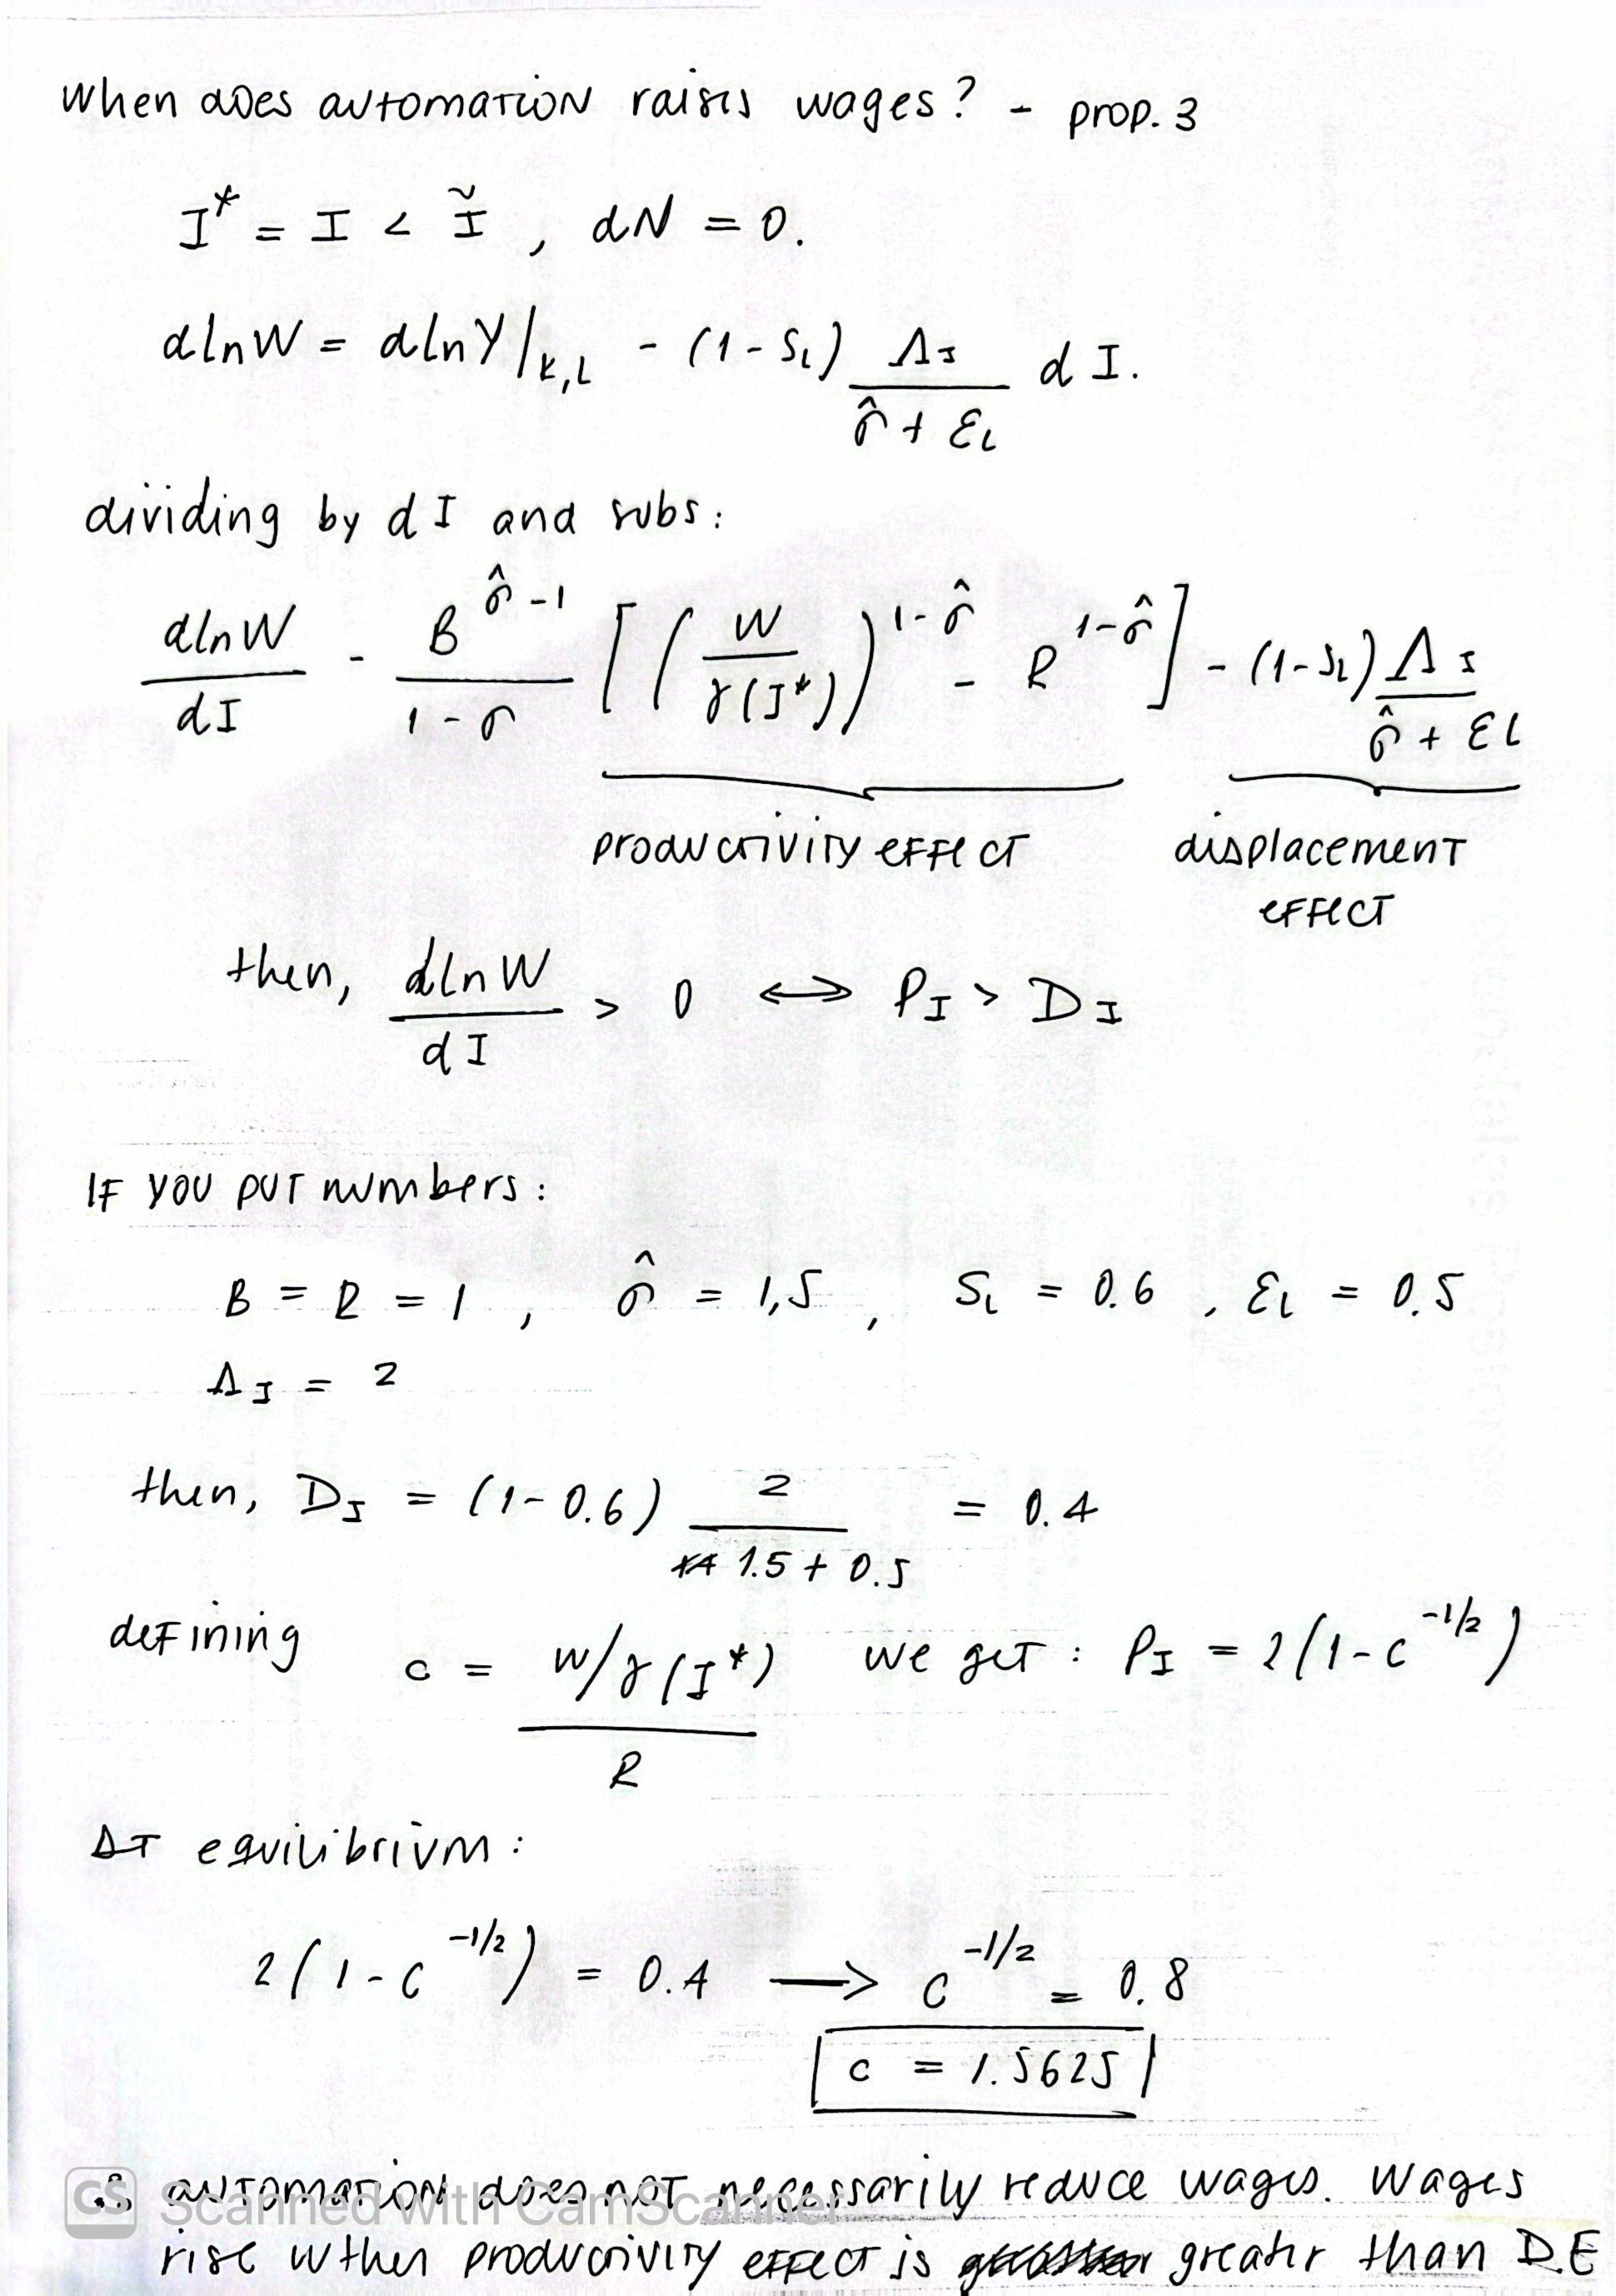
\includegraphics[height=2.0cm]{hand/wage-derivation.jpg}%
  }{%
    \colorbox{sand}{\parbox{0.95\textwidth}{\centering\small Owner-supplied photograph still required: \texttt{hand/wage-derivation.jpg}}}%
  }
  \source{Own hand derivation of Proposition 3; NBER pp. 12--14}
\end{frame}

\begin{frame}{What the model changes about the automation debate}
  \begin{itemize}
    \item Productivity gains do not determine the wage, employment, or labor share by themselves.
    \item Automation displaces labor from existing tasks. New tasks reinstate labor in the task frontier.
    \item The short-run wage effect is conditional on productivity gains relative to displacement.
    \item An interior innovation race can be stable, but full automation remains possible.
    \item Lean is useful here because every domain restriction and inequality must be stated explicitly.
  \end{itemize}

  \vfill
  {\small\color{rust}\texttt{github.com/amchavezu/ai-06-restrepo}}
\end{frame}

\end{document}
